% -*- mode: latex-mode; TeX-engine: xetex; LaTeX-command-style: (("" "SOURCE_DATE_EPOCH=0 %(PDF)%(latex) --shell-escape %S%(PDFout)")); TeX-master: "../dissertation.tex"; -*-

\chapter{Coherent Optical Creation of NaCs Molecule}
\label{ch:raman-transfer}

\section{Introduction}

\section{Raman Transition Beyond Three-Level Model}

In an ideal three-level system, the scattering probability during a $\pi$ pulse
can be arbitrarily small by using a large single photon detuning.
However, in practice, there are often other effects that increases the scattering
and may also put a lower limit on the minimum scattering probability during the transfer.
In this section, we will discuss the difference between an ideal Raman transition
in three-level system and on in a real system.

\subsection{Generic Model}

\ref{fig:raman-transfer-generic-raman-model}

\begin{figure}
  \centering
  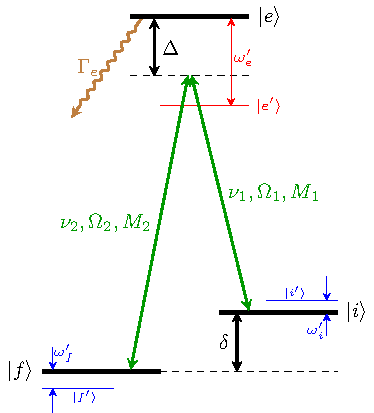
\includegraphics[width=0.6\textwidth]{figures/raman_transfer_generic_raman_model.pdf}
  \caption[Generic model for a real Raman transition]{
    \todo{}
    \label{fig:raman-transfer-generic-raman-model}}
\end{figure}

\todo{}

Due to experimental constraint,
we will discuss only in the limit where the single photon detuning is
much smaller than the frequency of each individual beams ($\Delta\ll\nu_1,\ \nu_2$).

\subsection{Additional Initial and Final States}

\subsection{Additional Excited states}

\subsection{Cross Coupling Between Light Addressing Initial and Final States}

\todo{Light shift?}

\section{Raman Transfer versus STIRAP}

An alternative method often used to create and prepare the internal states of ultracold molecule
is stimulated Raman adiabatic passage (STIRAP)\todo{\cite{}}.
Compared to off-resonance Raman transition, which uses detuning from the excited state
to reduce scattering during the transfer, STIRAP relies on a superposition between
the initial and final state as a dark state to achieve the same goal.
The dark state in STIRAP is created due to a destructive interference of transition
from the initial and final state to the excited state.

Similar to Raman transfer, STIRAP in an ideal three-level system can achieve
full coherent transfer with arbitrarily small scattering probability
when given unlimited time and power budget.
However, in reality, states and coupling that exist outside the ideal three-level system
always have a non-zero probability of scattering loss.
In this section, we will apply the approach we took for Raman transition
and apply it to STIRAP. We will then compare the loss caused by different practical limitations
and discuss which approach should be taken under certain circumstance.

% \subsection{Theory}

\subsection{Additional Initial and Final States}

\subsection{Additional Excited states}

\subsection{Cross Coupling Between Light Addressing Initial and Final States}

\subsection{Conclusion}

\section{States Selection}

(Differential Light Shift)
(Scattering)

\subsection{Excited State Selection}

\subsection{Ground States Selection}

\subsubsection{Final Molecular State}

\subsubsection{Initial Atomic State}

\section{Raman Transfer Results}

\subsection{Scaling of Raman Transition Parameters}
